% Ejemplo de documento LaTeX
% Tipo de documento y tamaño de letra
\documentclass[10pt]{article}
% Preparando para documento en Español.
% Para documento en Inglés no hay que hacer esto.
\usepackage[spanish]{babel}
\selectlanguage{spanish}
\usepackage[utf8]{inputenc}


% EL titulo, autor y fecha del documento
\title{Mareas y Series de tiempo}
\author{Rios Quijada Danira}
\date{07 de Mayo de 2015}
% Aqui comienza el cuerpo del documento
\usepackage{graphicx}
\begin{document}
% Construye el título
\maketitle
\section{Mareas}
La marea es el cambio periódico del nivel del mar producido principalmente por la fuerza de atracción gravitatoria que ejercen el Sol y la Luna sobre la Tierra.
\\ \space
El fenómeno de las mareas es conocido desde la antigüedad. Pero fue Isaac Newton en su obra Philosophiae Naturalis Principia Mathematica («Principios matemáticos de la Filosofía Natural», 1687) quien dio la explicación de las mareas aceptada actualmente. Más tarde, Pierre-Simon Laplace (1749-1827) y otros científicos ampliaron el estudio de las mareas desde un punto de vista dinámico.
\\ \space
Isaac Newton realizó varios estudios científicos del comportamiento de las mareas y calculó la altura de éstas según la fecha del mes, la estación del año y la latitud. Más tarde, Simon Laplace complementó los estudios de Newton.
\\
\\
\\
\section{Teoría de las mareas}
La teoría de las mareas es la aplicación de la mecánica de medios continuos para interpretar y predecir las deformaciones de cuerpos planetarios y satélites y sus atmósferas y océanos (especialmente del océano de la Tierra) en virtud de la carga gravitacional de otro cuerpo o cuerpos astronómicos (especialmente la Luna). \\ \space
Pierre-Simon Laplace en 1775, describe la reacción del océano a las fuerzas de marea. La teoría de las mareas oceánicas de Laplace tuvo en cuenta la fricción, la resonancia y los períodos naturales de las cuencas oceánicas. Predijo los grandes sistemas anfidrómicos en las cuencas oceánicas del mundo y explico las mareas oceánicas que se observan en la actualidad.  


\newpage
\section{Programa FORTRAN}

En esta ocasión diseñamos y creamos un programa que encontrara las mareas máximas y mínimas de cada mes, para después encontrar el periodo de las mareas máximas y mínimas; lo mismo hicimos con las mareas diarias. El código que utilizamos fue el siguiente:
\\
\begin{verbatim}  
 PROGRAM Mareas

IMPLICIT NONE
REAL, DIMENSION (7674):: altura
INTEGER :: i
!-------------------------------------
REAL :: Dif, Maxm1, Maxm2, Maxm3, Maxm4, Maxm5
REAL :: Tiempom1x, Tiempom2x, Tiempom3x, Tiempom4x, Tiempom5x
!-------------------------------------
REAL :: Dif2, Minm1, Minm2, Minm3, Minm4, Minm5
REAL :: Tiempom1n, Tiempom2n, Tiempom3n, Tiempom4n, Tiempom5n
!-------------------------------------
REAL :: Dif3, Maxd1, Maxd2, Maxd3, Maxd4, Maxd5
REAL :: Tiempod1x, Tiempod2x, Tiempod3x, Tiempod4x, Tiempod5x
!-------------------------------------
REAL :: Dif4, Mind1, Mind2, Mind3, Mind4, Mind5
REAL :: Tiempod1n, Tiempod2n, Tiempod3n, Tiempod4n, Tiempod5n
!-------------------------------------
REAL :: PeriodomM1, PeriodomM2, PeriodomM3, PeriodomM4, PeriodomM5
REAL :: PeriodomN1, PeriodomN2, PeriodomN3, PeriodomN4, Periodomn5
REAL :: PeriododM1, PeriododM2, PeriododM3, PeriododM4, PeriododM5
REAL :: PeriododN1, PeriododN2, PeriododN3, PeriododN4, PeriododN5
!--------------------------------------
REAL :: Periodo_mensual_max
REAL :: Periodo_mensual_min
REAL :: Periodo_diario_max
REAL :: Periodo_diario_min
!-------------------------------------




OPEN (1,file="Mareas.csv")

DO i=1,7674
READ (1,*) altura(i)
END DO
CLOSE (1)

Maxm1 = 0
DO i=1,1344
Dif=Maxm1 - altura(i)
IF (Dif < 0) THEN 
Maxm1 = altura (i)

Tiempom1x= i/48.0

END IF
END DO

Maxm2 = 0
DO i=1345,2690
Dif =  Maxm2 - altura(i)
IF (Dif < 0) THEN 
Maxm2 = altura(i)

Tiempom2x=i/48.0
END IF
END DO


Maxm3 = 0
DO i=2691,4035
Dif = Maxm3 - altura(i)
IF (Dif < 0) THEN 
Maxm3 = altura (i)

Tiempom3x=i/48.0
END IF
END DO 

Maxm4 = 0
DO i=4036,5380
Dif = Maxm4 - altura(i)
IF (Dif < 0) THEN 
Maxm4 = altura (i)

Tiempom4x=i/48.0
END IF
END DO

Maxm5 = 0
DO i=5381, 6725
Dif = Maxm5 - altura(i)
IF (Dif < 0) THEN 
Maxm5 = altura (i)

Tiempom5x=i/48.0
END IF
END DO

!---------------------------------------------

Minm1 = 0
DO i= 1, 1344
Dif2= Minm1 - altura(i)
IF (Dif2> 0) THEN 
Minm1 = altura (i)

Tiempom1n=i/48.0
END IF
END DO

Minm2 = 0
DO i= 1345, 2690
Dif2= Minm2 - altura(i)
IF (Dif2> 0) THEN 
Minm2 = altura (i)

Tiempom2n=i/48.0
END IF
END DO

Minm3 = 0
DO i= 2691, 4035
Dif2= Minm3 - altura(i)
IF (Dif2> 0) THEN 
Minm3 = altura (i)

Tiempom3n=i/48.0
END IF
END DO

Minm4 = 0
DO i= 4036, 5380
Dif2= Minm4 - altura(i)
IF (Dif2> 0) THEN 
Minm4 = altura (i)

Tiempom4n=i/48.0
END IF
END DO

Minm3 = 0
DO i= 5381, 6725
Dif2= Minm5 - altura(i)
IF (Dif2> 0) THEN 
Minm5 = altura (i)

Tiempom5n=i/48.0
END IF
END DO


!--------------------------------------------

Maxd1 = 0
DO i= 18, 65
Dif3= Maxd1- altura(i)
IF (Dif3< 0) THEN 
Maxd1 = altura (i)

Tiempod1x= i * 0.5

END IF
END DO

Maxd2 = 0
DO i= 66, 113
Dif2=  Maxd2 - altura(i)
IF (Dif3< 0) THEN 
Maxd2 = altura(i)

Tiempod2x=(i* 0.5)

END IF
END DO


Maxd3 = 0
DO i= 114, 161
Dif3= Maxd3 - altura(i)
IF (Dif3< 0) THEN 
Maxd3 = altura (i)

Tiempod3x=(i* 0.5)

END IF
END DO 

Maxd4 = 0
DO i= 162, 209
Dif3= Maxd4 - altura(i)
IF (Dif3< 0) THEN 
Maxd4 = altura (i)

Tiempod4x=(i* 0.5)

END IF
END DO 

Maxd5 = 0
DO i= 210, 257
Dif3= Maxd5 - altura(i)
IF (Dif3< 0) THEN 
Maxd5 = altura (i)

Tiempod5x=(i* 0.5)

END IF
END DO 

!--------------------------------------------

Mind1 = 0
DO i= 18, 65
Dif4= Mind1 - altura(i)
IF (Dif4> 0) THEN 
Mind1 = altura (i)

Tiempod1n=i * 0.5

END IF
END DO

Mind2 = 0
DO i= 66, 113
Dif4= Mind2 - altura(i)
IF (Dif2> 0) THEN 
Mind2 = altura (i)

Tiempod2n=( i * 0.5) 
END IF
END DO

Mind3 = 0
DO i= 114, 161
Dif4= Mind3 - altura(i)
IF (Dif4> 0) THEN 
Mind3 = altura (i)

Tiempod3n=(i* 0.5) 

END IF
END DO

Mind4 = 0
DO i= 162, 209
Dif4= Mind4 - altura(i)
IF (Dif4> 0) THEN 
Mind4 = altura (i)

Tiempod4n=(i* 0.5) 

END IF
END DO

Mind5 = 0
DO i= 210, 257
Dif4= Mind5 - altura(i)
IF (Dif4> 0) THEN 
Mind5 = altura (i)

Tiempod5n=(i* 0.5) 

END IF
END DO
!--------------------------------------------

PeriodomM1 = Tiempom1x 
PeriodomM2 = Tiempom2x - Tiempom1x
PeriodomM3 = Tiempom3x - Tiempom2x
PeriodomM4 = Tiempom4x - Tiempom3x
PeriodomM5 = Tiempom5x - Tiempom4x

PeriodomN1 = Tiempom1n 
PeriodomN2 = Tiempom2n - Tiempom1n
PeriodomN3 = Tiempom3n - Tiempom2n
PeriodomN4 = Tiempom4n - Tiempom3n
PeriodomN5 = Tiempom5n - Tiempom4n

PeriododM1 = Tiempod1x 
PeriododM2 = Tiempod2x - Tiempod1x
PeriododM3 = Tiempod3x - Tiempod2x
PeriododM4 = Tiempod4x - Tiempod3x
PeriododM5 = Tiempod5x - Tiempod4x

PeriododN1 = Tiempod1n 
PeriododN2 = Tiempod2n - Tiempod1n
PeriododN3 = Tiempod3n - Tiempod2n
PeriododN4 = Tiempod4n - Tiempod3n
PeriododN5 = Tiempod5n - Tiempod4n

!---------------------------------------------

Periodo_mensual_max = (PeriodomM1 + PeriodomM2 + PeriodomM3 + PeriodomM4 + PeriodomM5)/5.0

Periodo_mensual_min = (PeriodomN1 + PeriodomN2 + PeriodomN3 + PeriodomN4 + PeriodomN5)/5.0

Periodo_diario_max = (PeriododM1 +PeriododM2 +PeriododM3 + PeriododM4 + PeriododM5)/5.0

Periodo_diario_min = (PeriododN1 +PeriododN2 +PeriododN3 + PeriododN4 + PeriododN5)/5.0



Print *, '========================================================================'
Print *, 'Las mareas maximas mensuales fueron:'
Print *, '------------------------------------------'       
Print *, 'Primer mes:', Maxm1,'En el dia:', Tiempom1x
Print *, '------------------------------------------'
Print *, 'Segundo mes:',Maxm2,'En el dia:', Tiempom2x
Print *, '------------------------------------------'              
Print *, 'Tercer mes:',Maxm3,'En el dia:', Tiempom3x
Print *, '------------------------------------------'
Print *, 'Cuarto  mes:',Maxm4,'En el dia:', Tiempom4x
Print *, '------------------------------------------'              
Print *, 'Quinto mes:',Maxm5,'En el dia:', Tiempom5x
Print *, '========================================================================'
Print *, 'Las mareas minimas mensuales fueron:'
Print *, '------------------------------------------'       
Print *, 'Primer mes:',Minm1, 'En el dia:', Tiempom1n
Print *, '------------------------------------------'
Print *, 'Segundo mes:',Minm2,'En el dia:', Tiempom2n
Print *, '------------------------------------------'              
Print *, 'Tercer mes:',Minm3,'En el dia:', Tiempom3n
Print *, '------------------------------------------'
Print *, 'Cuarto  mes:',Minm4,'En el dia:', Tiempom4n
Print *, '------------------------------------------'              
Print *, 'Quinto  mes:',Minm5,'En el dia:', Tiempom5n
Print *, '========================================================================'
Print *, 'El periodo mensual de la  marea  maxima  es:', Periodo_mensual_max, 'dias'
Print *, '------------------------------------------------------------------'
Print *, 'El periodo mensual de la marea minima es:', Periodo_mensual_min, 'dias'
Print *, '========================================================================'
Print *, 'Las mareas maximas diarias fueron:'
Print *, '------------------------------------------'       
Print *, 'Primer dia:', Maxd1
Print *, '------------------------------------------'
Print *, 'Segundo dia:',Maxd2
Print *, '------------------------------------------'              
Print *, 'Tercer dia:',Maxd3
Print *, '------------------------------------------'
Print *, 'Cuarto dia:',Maxd4
Print *, '------------------------------------------'              
Print *, 'Quinto dia:',Maxd5
Print *, '========================================================================'
Print *, 'Las mareas minimas diarias fueron:'
Print *, '------------------------------------------'       
Print *, 'Primer dia:',Mind1
Print *, '------------------------------------------'
Print *, 'Segundo dia:',Mind2
Print *, '------------------------------------------'              
Print *, 'Tercer dia:',Mind3
Print *, '------------------------------------------'
Print *, 'Cuarto dia:',Mind4
Print *, '------------------------------------------'              
Print *, 'Quinto dia:',Mind5
Print *, '========================================================================'
Print *, 'El periodo diario de la marea maxima es:', Periodo_diario_max, 'hrs'
Print *, '------------------------------------------------------------------'
Print *, 'El periodo diario de la marea  minima es:', Periodo_diario_min, 'hrs' 
Print *, '========================================================================'


end program Mareas

\end{verbatim} 

\newpage
\subsection{Resultados}
Una vez compilado el programa, obtuvimos los siguientes resultados al correrlo.\\

\begin{tabular}{c}
\begin{center}
   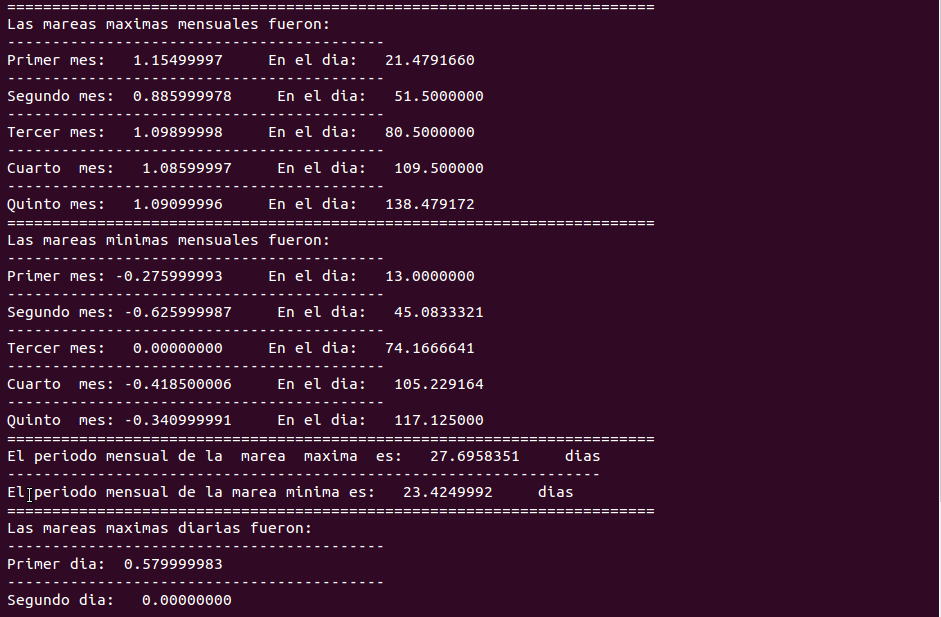
\includegraphics[scale=0.4]{mareasprint1.png}
\end{center}
\end{tabular}


\begin{tabular}{c}
\begin{center}
   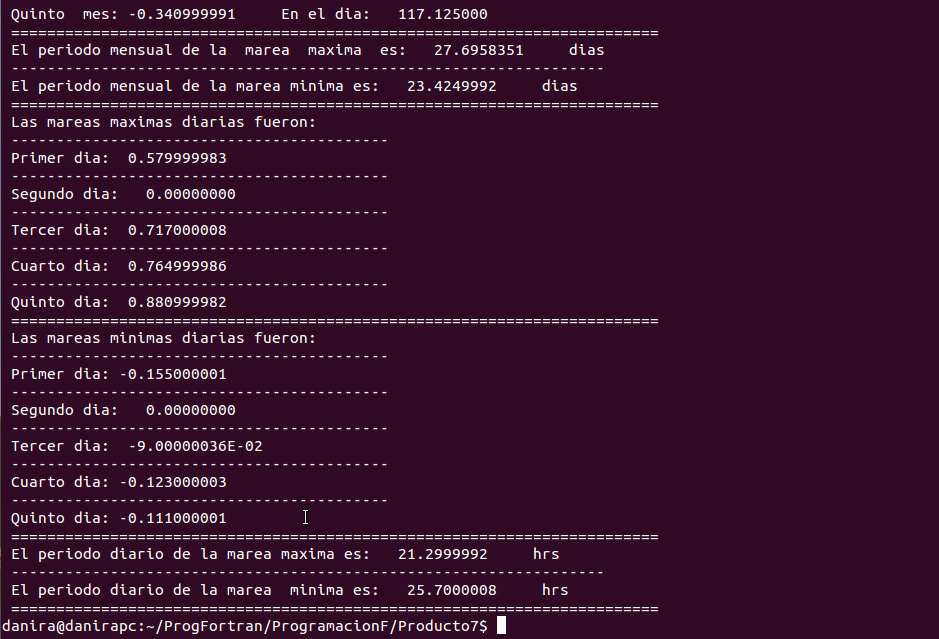
\includegraphics[scale=0.4]{mareasprint2.png}
\end{center}
\end{tabular}



\newpage


\section{Gráficas}
En la primera gráfica, se pueden observar todos los máximos y mínimos del total de datos, sin embargo no se pueden analizar los periódos.
\begin{center}
 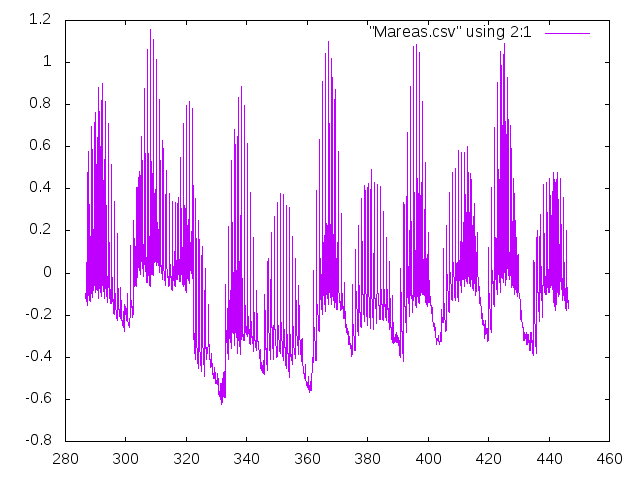
\includegraphics[scale=0.8]{grafica1.png}
\end{center}


\newpage
\subsection{Graficación por meses}
En las gráficas de cada mes se pueden detectar los máximos y mínimos de los mismos.
\begin{center}
   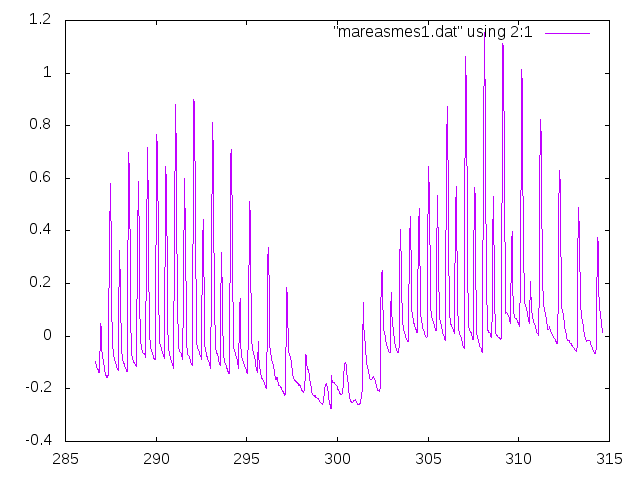
\includegraphics[scale=0.8]{month1.png}
\end{center}

\begin{center}
   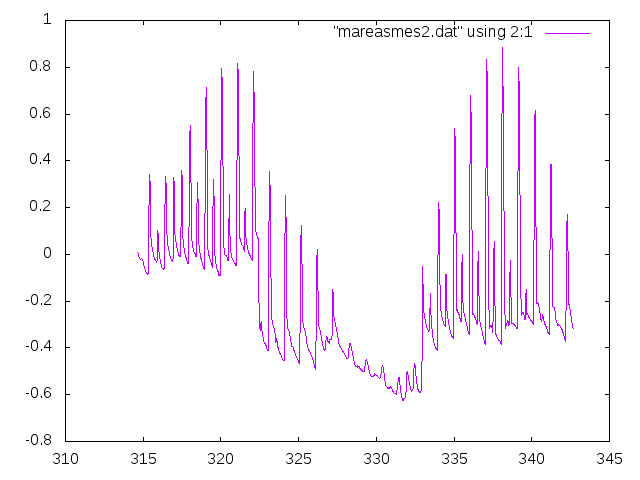
\includegraphics[scale=0.8]{month2.png}
\end{center}

\begin{center}
   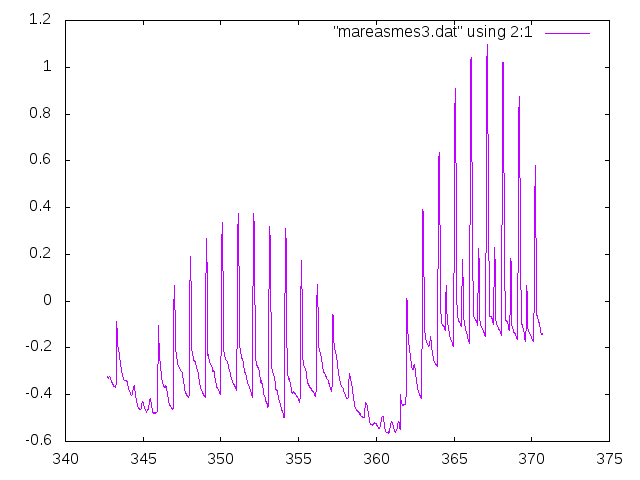
\includegraphics[scale=0.8]{month3.png}
\end{center}
\newpage
\subsection{Graficación por días}
En las gráficas de los días se puede analizar aproximadamente en que parte del día son las mareas más altas y más bajas.

\begin{center}
   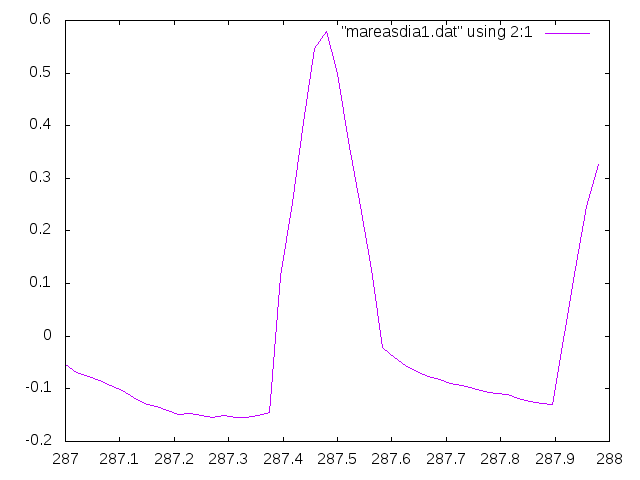
\includegraphics[scale=0.8]{day1.png}
\end{center}

\begin{center}
   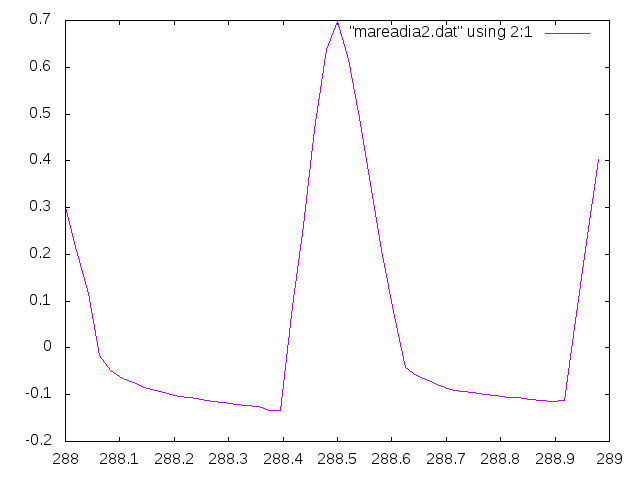
\includegraphics[scale=0.8]{day2.png}
\end{center}

\begin{center}
   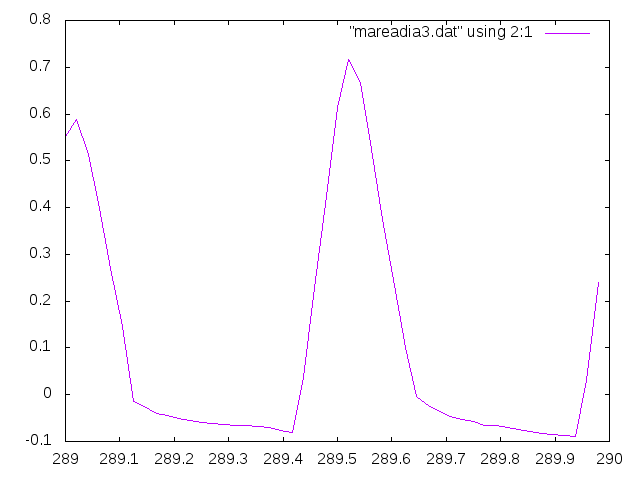
\includegraphics[scale=0.8]{day3.png}
\end{center}









% Nunca debe faltar esta última linea.
\end{document}
